\documentclass[a4paper,titlepage]{artikel1}
\usepackage[dutch]{babel}
%\usepackage{a4wide}
%\usepackage{eurofont}


\usepackage{ucs}
\usepackage[utf8x]{inputenc}
\usepackage{fullpage}
\usepackage{url}
\usepackage{eurosans} 
\usepackage{multirow}
\usepackage{graphicx}

\setlength{\parskip}{0.2cm}
\setcounter{secnumdepth}{3}


\author{Paul Sohier 0806122\\Sebastiaan Polderman 0820738}
\title{Automatisering}


\begin{document}
\maketitle
\tableofcontents
\newpage
 \section{Week 1}
  \subsection{Opdrachten bij hoofdstuk 1}
   \subsubsection[Opdracht 1]{Geef voorbeelden van computerprogramma's die voornamelijk ontwikkeld worden volgens het watervalmodel}
   Een pakket als MS Office zou volgens dit model ontwikkeld worden omdat het van te voren bepaalde eisen heeft aan de functionaliteit. 
   Zodra het basis pakket ontwikkeld is zal er niet veel meer veranderd worden aan het uitendelijke doel van het programma.
   
   \subsubsection[Opdracht 2]{Geef voorbeelden van computerprogramma's die voornamelijk ontwikkeld worden met prototyping.}
   Een goed voorbeeld hierbij is een project op school. Hierbij wordt eigenlijk bijna direct begonnen met het werken aan het eindproduct, terwijl er nog niet echt bedacht is wat het eindproduct moet worden. Op diverse punten tijdens de ontwikkeling van het programma zal het eisenpakket worden aangepast naar de uiteiendelijke wensen.
   
   \subsubsection[Opdracht 3]{Wat is het verschil tussen validatie en verificatie}
   Bij validatie (Valideren) wordt gekeken of het ontwerp voldoet aan het eisenpakket, terwijl er bij verificatie wordt gekeken of het process voldeed.
   
   \subsubsection[Opdracht 4]{Hoe zou u de ontwikkeltrajacten van het waterval-, het incremenetele- en het evolutionare model aangeven in figuur 1.1?}
   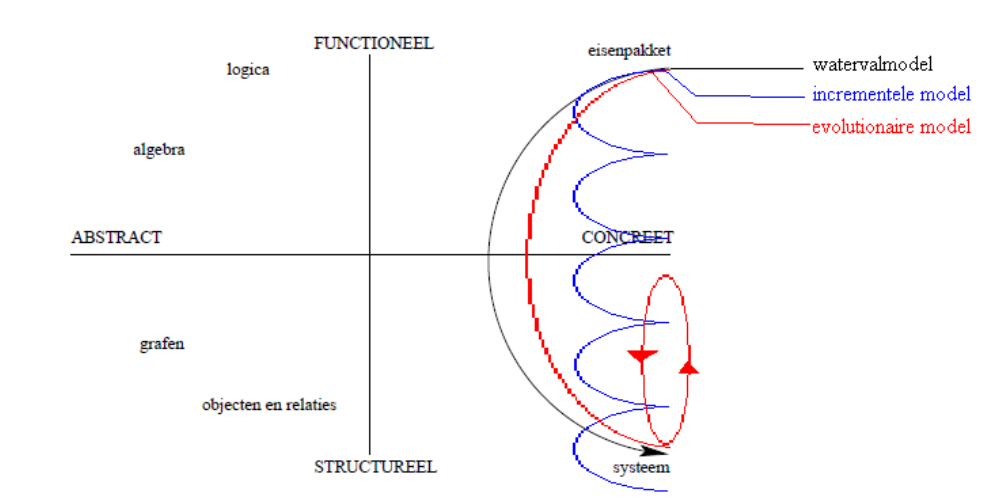
\includegraphics[scale=0.5]{H1O4.png}
   
   \subsubsection[Opdracht 5]{Zal de evolutionare ontwikkelstrategie de grens tussen ontwikkeling en onderhoud laten verdwijnen?}
   Ja, zodra je onderhoud doet kan je tegelijkertijd ook nieuwe, door de klant gewenste, features kunnen toevoegen aan het al bestaande programma. 
   
   \subsubsection[Opdracht 6]{Zoek op internet voorbeelde van repositories.}
   Een voorbeeld hiervan zijn de door debian gebruikte repositories, waaruit alle Debian installaties software vandaan installeren.
   
   \subsubsection[Opdracht 7]{Geef de voor en nadelen van open-source software.}
   Een groot voordeel is dat de sourcecode van de applicatie/programma vrijelijk te bekijken is. Hierdoor zie je dat bijvoorbeeld security problemen welke in deze source code aanwezig zijn sneller gevonden worden en hierdoor het algemener bekend is of software veilig is of niet.
   \\
   Helaas is dit grote voordeel ook direct een nadeel. Wanneer een security probleem gevonden wordt in een applicatie/programma en dit wordt niet opgelost door de vendor kan dit makkelijk misbruikt worden door de vaak uitgebreide verspreiding van de software. 
   \\ 
   Om dit probleem in het geheel op te lossen zal je dus een combinatie moeten maken tussen veilig gebruik van software (Kijkend naar de geschiedenis van software) en ander soort software.
   
   \subsubsection[Opdracht 8]{De eis ''Alle uitvoer moet normaal binnen 10 seconden gegeven worden'' is om \'{e}\'{e}n van de volgende redenen fout. Welke?}
   \begin{itemize}
    \item[a] Dubbelzinnig
    \item[b] Niet concreet
    \item[c] Tegenstrijdig
   \end{itemize}
   De eis is niet concreet genoeg, doordat alle uitvoer heel algemeen is. Een verbetering op deze eis zou zijn:\\
   ''De klant moet binnen 10 seconden een bevestiging van zijn bestelling op het scherm zien.''
   
   
   \subsubsection[Opdracht 9]{Wat mankeert er aan de eis: ''Het bestand moet een afsluitteken bevatten.''?}
   De eis is onduidelijk, doordat het afsluitteken niet is vastgesteld in de eis. 
   
   \subsubsection[Opdracht 10]{Welke maatregelen kunnen positief of negatief werken op:}
   \begin{itemize}
    \item[a] De correctheid
    \item[b] De beschikbaarheid
    \item[c] De herstelbaarheid
   \end{itemize}
   \begin{itemize}
     \item[a] Regelmatige validatie en verificatie tijdens alle stappen van het project.
     \item[b] Het systeem zo laten functioneren dat, mocht er een storing plaatsvinden in een bepaald gedeelte, dat de rest van het systeem nog naar behoren blijft functioneren.
     \item[c] Optimalisatie van de programmatuur.
   \end{itemize}
   
 \section{Week 2}
  \subsection{Opdrachten bij hoofdstuk 3}
   \subsubsection[Opdracht 1]{De projectkosten worden begroot op
   100000euro. De winst wordt gesteld op 15\%.Het risico dat men met dit
   project denkt te lopen, is gebaseerd op de ervaring dat 20\% van dit
   soort projecten mislukken. De BTW bedraagt 19\%. Hoeveel is de
   aanbestedingsprijs?}
   \begin{displaymath}
    (100*1.15*1.2)*1.19={164.20}euro
   \end{displaymath}
   
   \subsubsection[Opdracht 2]{Wat zijn de verschillen tussen kosten en investeringen?}
   Kosten zijn uitvagen die direct van de winst mogen worden afgetrokken. Inversteringen daarintegen moeten over meerdere jaren worden afgeschreven. Die jaarlijkse afschrijven mogen wel als kosten worden opgevoerd.
   
   \subsubsection[Opdracht 3]{Noem 3 investeringscriteria}
   \begin{itemize}
    \item Maximale gemiddelde boekhoudkundige rendabiliteit
    \item Minimale terugverdienperiode
    \item Concurrentievoordeel krijgen
   \end{itemize}
   \subsubsection[Opdracht 5]{Men kan een productiemiddel huren voor de
   prijs van 6100 e per maand. Indien men dit productiemiddel voor
   120000 e aanschaft, moet men 100 e per maand onderhoud betalen. De
   restwaarde is nihil.
   \begin{itemize}
     \item Bepaal het omslagpunt.
     \item Bereken het omslagpunt indien de discontovoet $1\%$ per maand is.
     \item Welke financiele overweging kan bij deze keuze een belangerijke rol spelen?
   \end{itemize}
   }
    \begin{itemize}
     \item Het omslagpunt:
	   \begin{displaymath}
	    \frac{120000}{(6100-100)}=20
	   \end{displaymath}
	   \\Het omslagpunt ligt dus bij 20 maanden
     \item Het omslagpunt bij een discotovoet van $1\%$ per maand
	   \begin{displaymath}
	    120000*1.01^{-20}=98345.34
	   \end{displaymath}
	   \begin{displaymath}
	    \frac{98345.34}{6100-100}=16.39
	   \end{displaymath}
	   \\
           Het omslagpunt ligt dan bij $16.36$ maanden.
     \item Welke overweging kan bij deze keuze een belangerijke rol spelen?\\De duurzaamheid of het gebruik van de inverstering. Hieruit bepaal je dan of het goedkoper is om te kopen of juist andersom.
    \end{itemize}
    
 \section{Week 3}
  \subsection{Opdrachten bij hoofdstuk 4}
   \subsubsection[Opdracht 1]{Noem minimaal 7 factoren die de individuele productiviteit be\"invloeden.}
   \begin{itemize}
    \item[1] Kennisniveau
    \item[2] Sfeer
    \item[3] Taalbeperkingen
    \item[4] Afhankelijk van hulpmiddelen
    \item[5] Budget
    \item[6] Werkprocessen
    \item[7] Beloning
   \end{itemize}
   
   \subsubsection[Opdracht 2]{Wat is het bezwaar tegen de definitie van
   individuele productiviteit: ``De omvang van de objectcode
   (gecompileerde programmatuur) in bytes per tijdseenheid''?}
   Iemand die minder efficient programeert levert volgens deze stelling beter werk af. Ook wordt er hiermee niet gekeken naar de complexiteit van de code.
   
   \subsubsection[Opdracht 3]{Verklaar waarom het coderen in de
   uitwerkingsfase meestal minder dan 10\% van de totale kosten van de levenscyclus bedraagt.}
   Door het gebruik van hulpmiddelen krimpt het coderingsaandeel.
   
   \subsubsection[Opdracht 4]{Verklaar hoe uit de COCOMO methoden blijkt dat de projecttijd niet afhankelijk is van het aantal programmeurs.}
   De geschatte projecttijd T wordt berekend door het aantal mensmaanden tot de macht c (Compactheid), vermenigvuldigt met $2,5$. Op basis hiervan wordt het minimum aantal benodigde mensen geschat. Het model rekent niet de projecttijd uit op basis van het aantal teamleden.

   \subsubsection[Opdracht 5]{Een administratief systeem van 9 netto
   functiepunten werd met een inspanning van 3 mensmaanden
   ontwikkeld. Is dit kenmerkend voor een administratief
   automatiseringsproject?}
   Volgens figuur 4.6 (Tabel \ref{reffig46}) in de reader is de gemiddelde productiviteit voor administatieve systemen $15,2$. De parameters van vraag 5 geven een productiviteit van $3$.

   \begin{center}
   \begin{table}[h] %hij zet hem op volgende pagina. Moet nog even kijken hoe beter aan te passen dat hij echt hier komt.
     \caption{Figuur 4.6}\label{reffig46}
     \begin{center}
     \begin{tabular}[t]{|l|l|l|l|}
       \hline
       \multirow{3}{*}{Toepassingsgebied} & \multicolumn{3}{c|}{Productiveit P [nfp/mensmaand]} \\
       \cline{2-4}
       & gemiddeld & standaarddeviatie & variatieco\"{e}ffici\"{e}nt \\
       & $\mu$ & $\sigma$ & $\rho$ \\
       \hline
       systemen met microcode & $1,5$ & $2,7$ & $1,80$ \\
       ingebedde realtime systemen & $6,8$ & $3,1$ & $0,46$ \\
       vliegtuigsystemen & $6,4$ & $3,3$ & $0,52$ \\
       commando en controle systemen & $9,9$ & $4,1$ & $0,41$ \\
       procesbesturings systemen & $10,3$ & $4,3$ & $0,42$ \\
       besturingsprogrammas en utilities & $11,3$ & $3,9$ & $0,35$ \\
       wetenschappelijke systemen & $12,5$ & $4,0$ & $0,32$ \\
       netwerksystemen & $10,3$ & $3,1$ & $0,30$ \\
       administratieve systemen & $15,2$ & $3,8$ & $0,24$ \\
       \hline
     \end{tabular}
     \end{center}
   \end{table}
   \end{center}
   
   \subsubsection[Opdracht 6]{Een computerprogramma heeft bij functiepuntanalyse voor de systeemkarakteristieken een totale correctiefactor $\bullet \begin{array}{c}14\\i=1 \end{array} c_i=50$. Uit de specificatie blijkt dat er 3 verschillende invoer-, 7 uitvoer- en 5 vraagtypen nodig zijn. Daarnaast zijn er 2 externe gegevensverzamelingen en 2 interne gegevensverzamelingen nodig. Alle geruiktsfuncties hebben een gemiddelde complexiteit. Men zal het computerprogramma coderen in de taal JAva ($C_t=53$). Er wordt geen gebruik gemaakt van hergebruik. Maak een schatting voor de broncode.}
   \begin{displaymath}
    f=3*4+4*5+5*4+2*10+2*7=12+20+20+20+14=86
   \end{displaymath}
   
   \begin{displaymath}
    NFP=(0,65+0,01*50)*86=98,9 %Was 1.15
   \end{displaymath}
   
   \begin{displaymath}
    S=98,9*53=5241,7
   \end{displaymath}
   Het aantal regels broncode is dus ongeveer $5241$
   \subsubsection[Opdracht 7]{Verklaar waarom juist computertalen met een lage ct waarde (zie paragraaf 4.1.1) geschikt zijn voor prototyping.}
   Dit komt doordat de hoeveelheid code kleiner is en hierdoor dus sneller is aan te passen
   
   \subsubsection[Opdracht 8]{Gegven een studentinformatiesysteem bestaande uit de volgende onderdelen:
     \begin{center}
   \begin{tabular}[t]{|ll|l|}
     \hline
     soort & omschrijving & complexiteit \\
     \hline
     module & inschrijving student & gemakkelijk \\
     module & uitschrijving student & gemakkelijk \\
     module & rekening collegegeld sturen & gemakkelijk \\
     module & machtiging betaling collegegeld verwerken & makkelijk \\
     module & betaling collegegeld verwerken & gemiddeld \\
     module & aanmaningen sturen & gemakkelijk \\
     module & tentamencijfers verwerken & moeilijk \\
     module & studieresultaten naar Informatie Beheer Groep & gemiddeld \\
     scherm & inschrijven van een student & gemiddeld \\
     scherm & uitschrijven van een student & gemiddeld \\
     scherm & betaling student invoeren & gemiddeld \\
     scherm & machtiging betaling invoeren & gemiddeld \\
     scherm & tentamencijfers invoeren & moeilijk \\
     scherm & vakkentabel invoeren & gemiddeld \\
     scherm & vakkentabel wijzigen & moeilijk \\
     formulier & studentgegevens & gemiddeld \\
     formulier & jaarlijkse voortgangsrapportage & moeilijk \\
     formulier & rapportage van tentamenresultaten & moeilijk \\
     formulier & aanmaningen collegegeld & gemiddeld \\
     \hline
   \end{tabular}
   \end{center}
   \begin{itemize}
     \item Maak met een objectpuntanalyse (OPA) een schatting voor de inspanning E als het hergebruik rond de $30\%$ ligt en het ontwikkelteam een lage productiviteit heeft. Maak een schatting met COCOMO-81 van de projecttijd T, indien het project een `organische' karakter heeft.
     \item Maak een schatting van de projecttijd T met COCOMO-II, indien er geen sprake is van tijdsdruk en het project de volgende karateristieken heeft:\\
       \begin{center}
       \begin{tabular}[]{|l|l|}
         \hline
         Karakteristieken & $b_i$ \\
         \hline
         ontwerpervaring & $0,05$ \\
         ontwerpvrijheid & $0,02$ \\
         ontwerprisico & $0,3$ \\
         ontwerpteam & $0,03$ \\
         organisatie & $0,01$ \\
         \hline
       \end{tabular}
       \\
       \end{center}
   \end{itemize}
   %\\ %Anders lijkt het antwoord op de vraag nog :)
   }
   \begin{itemize}
    \item OPA
	  \begin{displaymath}
	   NOP=50*(1-0.3)=35
	  \end{displaymath} 
	  \begin{displaymath}
	   E=\frac{35}{7}=5
	  \end{displaymath}
    \item COCOMO-81
	  \begin{displaymath}
	   T=2.5*5.2^{0.38}=4.78
	  \end{displaymath}
    \item COCOMO-II
	  \begin{displaymath}
	   T=(2.5*5.2^{0.33+0.2*0.14})=4.51
	  \end{displaymath}
   \end{itemize}
   \section{Week 4}

   \subsection{Opdrachten bij hoofdstuk 5}
   \subsubsection[Opdracht 1]{Gegeven een netwerk met 7 activiteiten:}
   \begin{center}
     \begin{tabular}{|l|l|l|l|l|l|}
       \hline
       activiteit & omschrijving & afhankelijk van & $t_b$ & $t_m$ & $t_w$ \\
       \hline
       A & Definitie & & 1 & 2 & 3 \\
       B & Hardware specificatie & A & 3 & 4 & 5 \\
       C & Software specificatie & A & 1 & 2 & 9 \\
       D & Hardware ontwikkeling & B & 1 & 2 & 3 \\
       E & Software ontwikkeling & B C & 4 & 5 & 12 \\
       F & Documenteren & D & 3 & 4 & 5 \\
       G & Systeemintergratie & D E & 3 & 3 & 3 \\
       \hline
     \end{tabular}
   \end{center}
   \begin{itemize}
     \item[a] Bepaal met PERT het mijpalenplan en het kritieke pad
     \item[b] Bepaal het Ganttscheme. Welke conclusies kan men daaruit trekken?
     \item[c] Bepaal het 95\%-betrouwbaarheidsinterval voor de werkelijke projecttijd.
   \end{itemize}
   \begin{itemize}
     \item[a] Zie figuur \ref{r51a}.
     \item[b] Zie tabel \ref{r51b}.
     \item[c]
       \begin{displaymath}
         o²=2+2+8+2=2+8+2+0=24
       \end{displaymath}
       \begin{displaymath}
         14-(1,96*\sqrt{24})=<T=<14+(1,96*\sqrt{24}))
       \end{displaymath}
       \begin{displaymath}
         4,40=<T=<26,60
       \end{displaymath}
   \end{itemize}
       \begin{figure}[tbh]
         \caption{Antwoord bij Hoofdstuk 5 Vraag 1.a} \label{r51a}
         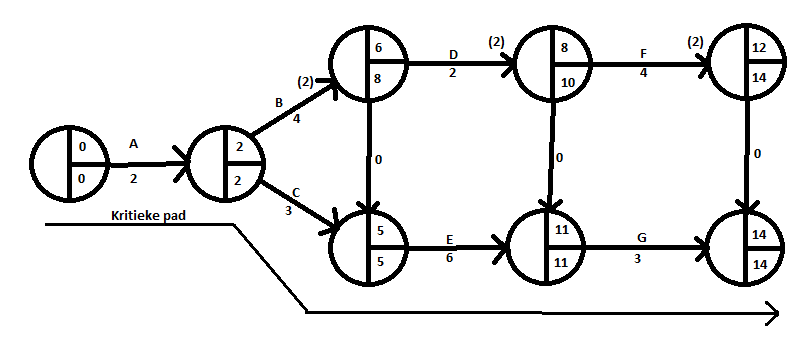
\includegraphics[scale=0.75]{H5O1A.png}     
       \end{figure}
   \begin{table}
     \caption{Antwoord bij Hoofdstuk 5 vraag 1.b} \label{r51b}
       \begin{tabular}[htb]{|l|l|l|l|l|l|l|l|l|l|l|l|l|l|l|}
         \hline
             & 0..1 & 1..2 & 2..3 & 3..4 & 4..5 & 5..6 & 6..7 & 7..8 & 8..9 & 9..10 & 10..11 & 11..12 & 12..13 & 13..14 \\
         \hline
         A 2 &  --- &  --- &      &      &      &      &      &      &      &       &        &        &        &\\
         \hline
         B 4 &      &      &  --- & ---  & ---  & ---  & - - -& - - -&      &       &        &        &        &\\
         \hline
         C 3 &      &      &  --- & ---  & ---  &      &      &      &      &       &        &        &        &\\
         \hline
         D 2 &      &      &      &      &      &      & - - -& - - -&      &       &        &        &        &\\
         \hline
         E 6 &      &      &      &      &      & ---  & ---  & ---  & ---  & ---   & ---    &        &        &\\
         \hline     
         F 4 &      &      &      &      &      &      &      &      & - - -& - - - & ---    & ---    & - - -  & - - -\\
         \hline
         G 3 &      &      &      &      &      &      &      &      &      &       &        & ---    & ---    & ---\\
         \hline
       \end{tabular}
   \end{table}
   
   \subsubsection[Opdracht 2]{bepaal van de volgend activiteiten met PERT het mijlpalenplan en een schatting van het kritieke pad $T_k$}
   \begin{center}
     \begin{tabular}{|l|l|l|}
     \hline
     activiteit & $t$ & afhankelijk van \\
     \hline
     A & 2 & K \\
     B & 3 & H \\
     C & 4 &\\
     D & 2 & F G \\
     E & 1 & D I J \\
     F & 3 & B \\
     G & 3 & C K \\
     H & 3 & \\
     I & 2 & A F \\
     J & 1 & F \\
     K & 2 & H \\
     \hline
     \end{tabular}
   \end{center}
   \subsubsection[Opdracht 3]{Van een collectief team is gegeven dat de verliesfactor per communicatiekaneel 5\% is, bereken de maximale groepsgrootte}
   \begin{displaymath}
     N=\frac{(1+i)}{(2*i)}=\frac{1+0,05}{2*0,05}=\frac{1,05}{0,10}=10,5
   \end{displaymath}

   \subsubsection[Opdracht 4]{Toon aan dat de volgende formule geldt voor het hi\"{e}rarchieke team met $N$ teamleden en maximaal 6 ondergeschikten per echelon:}
   \begin{displaymath}
     \lfloor^6\log{(5N+1)}\rfloor\leq echelons\leq N
   \end{displaymath}

   \section{Week 5}
   \subsection{Opdrachten bij hoofdstuk 7}
   \subsubsection[Opdracht 1]{Van een objectgeori\"{e}nteerd computerprogramma in Java, zijn van alle classes de metrieken NOM,CBO, RFC, WMC, DIT en NOC gemeten. Een tiental classes had een verhoogd risico.}
   \begin{itemize}
     \item[a] Maak een tabel met riskante waarden van de waarden van de metrieken.
       \begin{center}
         \begin{tabular}{|l|p{5cm}|l|l|}
           \hline
           Metrieken & Riskante waarde & reader bladzijde & reader paragraaf\\
           \hline
           NOM & Java gemiddeld: $\approx8$ & 84 & 7.2.2 \\
           & C++ gemiddeld: $\approx25$ & & \\
           & Kritiek: $>40$ & & \\
           \hline
           CBO & 5 & 86 & 7.2.5 \\
           \hline
           RFC & $\geq50$ & 87 & 7.2.7 \\
           \hline 
           RFC/NOM & Java: $\geq10$ & 88 & 7.2.7 \\
           & C++: $\geq5$ & & \\
           \hline
           WMC & aanbevolen: $\geq25$ & 83 & 7.2.1 \\
           & kritiek: $>75$ & & \\
           \hline
           DIT & 5 & 84  & 7.2.3 \\
           \hline
           NOC & Geen aanbevolen waarde, hoge NOC geeft slechte metriek & 85  & 7.2.4  \\
           \hline
         \end{tabular}
       \end{center}
     \item[b] Geef in de volgende tabel bij elke class aan welke metriek een kritieke waarde heeft. \\
       \begin{center}
       \begin{tabular}{|l|l|l|l|l|l|l|l|}
         \hline
         class & NOM & CBO & RFC & RFC/NOM & WMC & DIT & NOC \\
         \hline
         1 & 54 & 8 & 536 & 9,9 & 175 & 1 & 0 \\
         2 & 7 & 6 & 168 & 24,0 & 71 & 4 & 0 \\
         3 & 33 & 4 & 240 & 7,2 & 105 & 2 & 0 \\
         4 & 54 & 8 & 381 & 6,7& 117 & 2 & 2 \\
         5 & 62 & 6 & 378 & 6,1 & 163 & 2 & 0 \\
         6 & 63 & 7 & 235 & 3,7 & 156 & 2 & 0 \\
         7 & 81 & 10  & 285 & 3,5 & 161 & 2 & 0 \\
         8 & 42 & 5 & 127 & 3,0 & 69 & 3 & 0 \\
         9 & 20 & 17 & 325 & 16,2 & 139 & 4 & 4 \\
         10 & 46 & 5 & 186 & 4,0 & 238 & 1 & 3 \\
         \hline
       \end{tabular}
       \end{center}
       
       Bij NOC is er geen aanbevolen kritieke waarde, maar er is wel hoe hoger deze waarde is hoe slechter de metriek is. Wij hebben bij een NOC van $\geq3$ aangenomen dat de NOC kritiek is. Dit baseren wij op dat de NOC is gebaseerd op het aantal kinderen een class heeft, en hoe meer kinderen, hoe groter de kans op fout. Bij $\geq3$ is de kans op fouten volgens onze mening zeer goed aanwezig.\\
       Wanneer een waarde kritiek is voor een bepaald metriek, staat er in onderstaande tabel \begin{em}kritiek\end{em}. Wanneer er niets staat is de waarde niet kritiek. Er is uitgegaan dat de classes zijn geschreven in de taal JAVA. Indien de waarde uitmaakt voor de kritieke waarde, en de kritieke waarde voor C++ anders is, staat dit tussen haakjes. \\ 
         De waarde voor RFC is in alle gevallen kritiek. De waarde ligt flink boven de aangegeven kritieke waarde, welke tevens ook zeer hoog boven de kritieke waarde ligt. De kritieke waarde voor RFC ic $\geq50$, terwijl de laagste waarde voor RFC van de classes 127 is. \\
         De waarde voor DIT ligt in alle gevallen onder de kritieke waarde van 5. 
       \begin{center}
       \begin{tabular}{|l|l|l|l|l|l|l|l|}
         \hline
         class & NOM & CBO & RFC & RFC/NOM & WMC & DIT & NOC \\
         \hline
         1 & kritiek & kritiek & kritiek & (kritiek) & kritiek &  &  \\
         2 &  & kritiek & kritiek & kritiek(kritiek) &  &  &  \\
         3 &  &  & kritiek & (kritiek) & kritiek &  & \\
         4 & kritiek & kritiek & kritiek & (kritiek)& kritiek &  &  \\
         5 & kritiek & kritiek & kritiek & (kritiek) & kritiek &  &  \\
         6 & kritiek & kritiek & kritiek &  & kritiek &  &  \\
         7 & kritiek & kritiek  & kritiek &  & kritiek &  &  \\
         8 & kritiek & kritiek & kritiek &  &  &  &  \\
         9 &  & kritiek & kritiek & kritiek(kritiek) & kritiek &  & kritiek \\
         10 & kritiek & kritiek & kritiek &  & kritiek &  & kritiek \\
         \hline
       \end{tabular}
       \end{center}

   \end{itemize}
   
   \subsubsection[Opdracht 2]{Bepaald WMC, DIT, NOC, CBO, RFC en LCOM van de volgende pseudo objecten broncode:}
   \begin{center}
   \begin{tabular}[t]{|l|l|}
     \hline
     Class & trade \\
     Variables & trade.id, counterparty, trade\_value \\
     Methods & evaluate\_counterpart() \\
     & get\_trade\_id(trade\_id) \\
     & position\_update() \\
     & \{position\_manager::report\_trade()\} \\
     \hline
     Class & bond\_trade \\
     Variables & bond\_detials \\
     Methods & get\_bond\_info() \\
     \hline
     Class & fx\_trade \\
     Variables & forex\_detials \\
     Methods & calculate\_exchange\_rates() \\
     \hline
     Class & equity\_trade \\
     Variables & company, stock\_market, PE\_ratio,  earnings, week\_hi\_lo \\
     Methods & Estimate\_beta() \\
     & get\_stock\_quotes() \\
     & \{quotron::quotes()\} \\
     \hline
     Class &municipal\_bond\_trade \\
     Variables & state\_or\_federal, over\_the\_counter \\
     Methods & calculate\_coupon\_rate() \\
     & \{Tbil\_server::rate()\} \\
     \hline
     Class & corporate bond\_trade \\
     Variables & adr, sp\_rating \\
     Methods & calc\_rating(sp\_rating) \\
     & \{if adr then fx\_trade::calculate\_exchange\_rates()\} \\
     \hline
     Class & international\_equity \\
     Variables & exchange\_rate, quitation \\
     Methods & perform\_anaylysis\_roa()\\
     & \{fx\_trade::calculate\_exchange\_rates()\}\\
     & get\_quotron(quotation) \\
     \hline
     Class & domestic\_equity \\
     Variables & variables: attribute1\\
     Methods & \\
     \hline
   \end{tabular}
   \end{center}
\end{document}
